\documentclass[twoside]{book}

% Packages required by doxygen
\usepackage{calc}
\usepackage{doxygen}
\usepackage{graphicx}
\usepackage[utf8]{inputenc}
\usepackage{makeidx}
\usepackage{multicol}
\usepackage{multirow}
\usepackage{textcomp}
\usepackage[table]{xcolor}

% Font selection
\usepackage[T1]{fontenc}
\usepackage{mathptmx}
\usepackage[scaled=.90]{helvet}
\usepackage{courier}
\usepackage{amssymb}
\usepackage{sectsty}
\renewcommand{\familydefault}{\sfdefault}
\allsectionsfont{%
  \fontseries{bc}\selectfont%
  \color{darkgray}%
}
\renewcommand{\DoxyLabelFont}{%
  \fontseries{bc}\selectfont%
  \color{darkgray}%
}

% Page & text layout
\usepackage{geometry}
\geometry{%
  a4paper,%
  top=2.5cm,%
  bottom=2.5cm,%
  left=2.5cm,%
  right=2.5cm%
}
\tolerance=750
\hfuzz=15pt
\hbadness=750
\setlength{\emergencystretch}{15pt}
\setlength{\parindent}{0cm}
\setlength{\parskip}{0.2cm}
\makeatletter
\renewcommand{\paragraph}{%
  \@startsection{paragraph}{4}{0ex}{-1.0ex}{1.0ex}{%
    \normalfont\normalsize\bfseries\SS@parafont%
  }%
}
\renewcommand{\subparagraph}{%
  \@startsection{subparagraph}{5}{0ex}{-1.0ex}{1.0ex}{%
    \normalfont\normalsize\bfseries\SS@subparafont%
  }%
}
\makeatother

% Headers & footers
\usepackage{fancyhdr}
\pagestyle{fancyplain}
\fancyhead[LE]{\fancyplain{}{\bfseries\thepage}}
\fancyhead[CE]{\fancyplain{}{}}
\fancyhead[RE]{\fancyplain{}{\bfseries\leftmark}}
\fancyhead[LO]{\fancyplain{}{\bfseries\rightmark}}
\fancyhead[CO]{\fancyplain{}{}}
\fancyhead[RO]{\fancyplain{}{\bfseries\thepage}}
\fancyfoot[LE]{\fancyplain{}{}}
\fancyfoot[CE]{\fancyplain{}{}}
\fancyfoot[RE]{\fancyplain{}{\bfseries\scriptsize Generated on Fri Apr 22 2016 18\-:54\-:37 for My Project by Doxygen }}
\fancyfoot[LO]{\fancyplain{}{\bfseries\scriptsize Generated on Fri Apr 22 2016 18\-:54\-:37 for My Project by Doxygen }}
\fancyfoot[CO]{\fancyplain{}{}}
\fancyfoot[RO]{\fancyplain{}{}}
\renewcommand{\footrulewidth}{0.4pt}
\renewcommand{\chaptermark}[1]{%
  \markboth{#1}{}%
}
\renewcommand{\sectionmark}[1]{%
  \markright{\thesection\ #1}%
}

% Indices & bibliography
\usepackage{natbib}
\usepackage[titles]{tocloft}
\setcounter{tocdepth}{3}
\setcounter{secnumdepth}{5}
\makeindex

% Hyperlinks (required, but should be loaded last)
\usepackage{ifpdf}
\ifpdf
  \usepackage[pdftex,pagebackref=true]{hyperref}
\else
  \usepackage[ps2pdf,pagebackref=true]{hyperref}
\fi
\hypersetup{%
  colorlinks=true,%
  linkcolor=blue,%
  citecolor=blue,%
  unicode%
}

% Custom commands
\newcommand{\clearemptydoublepage}{%
  \newpage{\pagestyle{empty}\cleardoublepage}%
}


%===== C O N T E N T S =====

\begin{document}

% Titlepage & ToC
\hypersetup{pageanchor=false}
\pagenumbering{roman}
\begin{titlepage}
\vspace*{7cm}
\begin{center}%
{\Large My Project }\\
\vspace*{1cm}
{\large Generated by Doxygen 1.8.6}\\
\vspace*{0.5cm}
{\small Fri Apr 22 2016 18:54:37}\\
\end{center}
\end{titlepage}
\clearemptydoublepage
\tableofcontents
\clearemptydoublepage
\pagenumbering{arabic}
\hypersetup{pageanchor=true}

%--- Begin generated contents ---
\chapter{Hierarchical Index}
\section{Class Hierarchy}
This inheritance list is sorted roughly, but not completely, alphabetically\-:\begin{DoxyCompactList}
\item \contentsline{section}{Abstract\-Cell}{\pageref{classAbstractCell}}{}
\begin{DoxyCompactList}
\item \contentsline{section}{Conway\-Cell}{\pageref{classConwayCell}}{}
\item \contentsline{section}{Fredkin\-Cell}{\pageref{classFredkinCell}}{}
\end{DoxyCompactList}
\item \contentsline{section}{Cell}{\pageref{classCell}}{}
\item \contentsline{section}{Life$<$ T $>$}{\pageref{classLife}}{}
\end{DoxyCompactList}

\chapter{Class Index}
\section{Class List}
Here are the classes, structs, unions and interfaces with brief descriptions\-:\begin{DoxyCompactList}
\item\contentsline{section}{\hyperlink{classAbstractCell}{Abstract\-Cell} }{\pageref{classAbstractCell}}{}
\item\contentsline{section}{\hyperlink{classCell}{Cell} }{\pageref{classCell}}{}
\item\contentsline{section}{\hyperlink{classConwayCell}{Conway\-Cell} }{\pageref{classConwayCell}}{}
\item\contentsline{section}{\hyperlink{classFredkinCell}{Fredkin\-Cell} }{\pageref{classFredkinCell}}{}
\item\contentsline{section}{\hyperlink{classLife}{Life$<$ T $>$} }{\pageref{classLife}}{}
\end{DoxyCompactList}

\chapter{Class Documentation}
\hypertarget{classAbstractCell}{\section{Abstract\-Cell Class Reference}
\label{classAbstractCell}\index{Abstract\-Cell@{Abstract\-Cell}}
}
Inheritance diagram for Abstract\-Cell\-:\begin{figure}[H]
\begin{center}
\leavevmode
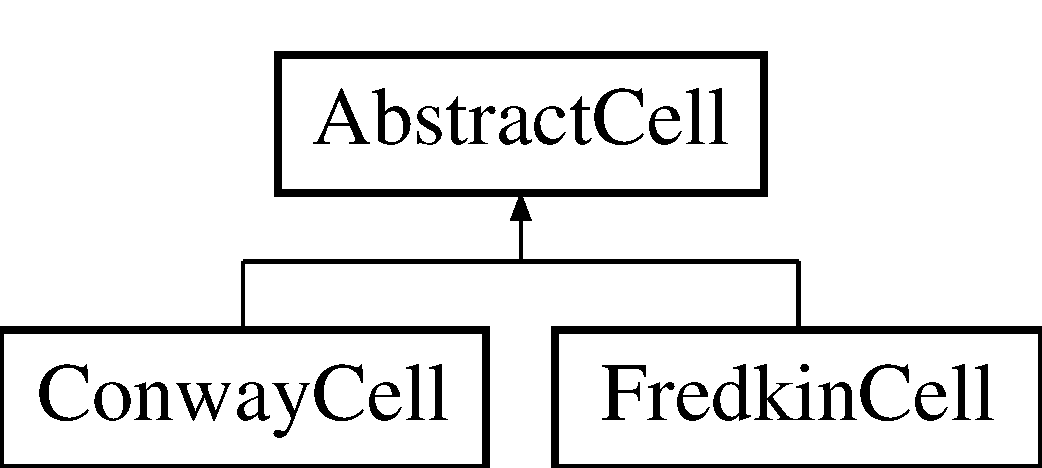
\includegraphics[height=2.000000cm]{classAbstractCell}
\end{center}
\end{figure}
\subsection*{Public Types}
\begin{DoxyCompactItemize}
\item 
enum {\bfseries Cell\-Type} \{ {\bfseries C\-O\-N\-W\-A\-Y}, 
{\bfseries F\-R\-E\-D\-K\-I\-N}
 \}
\end{DoxyCompactItemize}
\subsection*{Public Member Functions}
\begin{DoxyCompactItemize}
\item 
\hyperlink{classAbstractCell_acb4a116b1a007c03ce4e3644e6815a12}{Abstract\-Cell} ()
\item 
bool \hyperlink{classAbstractCell_a745364f521c5f2166387c36948f1d225}{is\-Alive} ()
\item 
virtual void \hyperlink{classAbstractCell_a2adb986c55c4ed6613549ff011fb8d25}{flip} ()
\item 
\hypertarget{classAbstractCell_a7902ac8171634af98039871fcd6ef8f8}{virtual void {\bfseries step} (int)=0}\label{classAbstractCell_a7902ac8171634af98039871fcd6ef8f8}

\item 
\hypertarget{classAbstractCell_abbc8049ebc500651020b0a9deb32726a}{virtual void {\bfseries print} () const =0}\label{classAbstractCell_abbc8049ebc500651020b0a9deb32726a}

\item 
\hypertarget{classAbstractCell_af28a8dcd6a7ac989c1fb85b06e254c90}{virtual void {\bfseries read} (char)=0}\label{classAbstractCell_af28a8dcd6a7ac989c1fb85b06e254c90}

\item 
\hypertarget{classAbstractCell_aa43ebbf6e33388ef444089328d6e3d99}{virtual int {\bfseries get\-Cell\-Type} () const =0}\label{classAbstractCell_aa43ebbf6e33388ef444089328d6e3d99}

\item 
\hypertarget{classAbstractCell_a6fd8f93b5a1547280fec2cb74241af38}{virtual \hyperlink{classAbstractCell}{Abstract\-Cell} $\ast$ {\bfseries clone} ()=0}\label{classAbstractCell_a6fd8f93b5a1547280fec2cb74241af38}

\end{DoxyCompactItemize}
\subsection*{Protected Attributes}
\begin{DoxyCompactItemize}
\item 
\hypertarget{classAbstractCell_aa92e42d5bb67f3249d8e2dde2c3228e7}{bool {\bfseries alive}}\label{classAbstractCell_aa92e42d5bb67f3249d8e2dde2c3228e7}

\item 
\hypertarget{classAbstractCell_aba7283aea356ed705101810b1623ca95}{bool {\bfseries to\-Flip}}\label{classAbstractCell_aba7283aea356ed705101810b1623ca95}

\end{DoxyCompactItemize}


\subsection{Constructor \& Destructor Documentation}
\hypertarget{classAbstractCell_acb4a116b1a007c03ce4e3644e6815a12}{\index{Abstract\-Cell@{Abstract\-Cell}!Abstract\-Cell@{Abstract\-Cell}}
\index{Abstract\-Cell@{Abstract\-Cell}!AbstractCell@{Abstract\-Cell}}
\subsubsection[{Abstract\-Cell}]{\setlength{\rightskip}{0pt plus 5cm}Abstract\-Cell\-::\-Abstract\-Cell (
\begin{DoxyParamCaption}
{}
\end{DoxyParamCaption}
)}}\label{classAbstractCell_acb4a116b1a007c03ce4e3644e6815a12}
Creates a cell 

\subsection{Member Function Documentation}
\hypertarget{classAbstractCell_a2adb986c55c4ed6613549ff011fb8d25}{\index{Abstract\-Cell@{Abstract\-Cell}!flip@{flip}}
\index{flip@{flip}!AbstractCell@{Abstract\-Cell}}
\subsubsection[{flip}]{\setlength{\rightskip}{0pt plus 5cm}void Abstract\-Cell\-::flip (
\begin{DoxyParamCaption}
{}
\end{DoxyParamCaption}
)\hspace{0.3cm}{\ttfamily [virtual]}}}\label{classAbstractCell_a2adb986c55c4ed6613549ff011fb8d25}
Flips the alive flag of the cell 

Reimplemented in \hyperlink{classFredkinCell_a0a849ac1b7b8620429b2f5c139043e87}{Fredkin\-Cell}.

\hypertarget{classAbstractCell_a745364f521c5f2166387c36948f1d225}{\index{Abstract\-Cell@{Abstract\-Cell}!is\-Alive@{is\-Alive}}
\index{is\-Alive@{is\-Alive}!AbstractCell@{Abstract\-Cell}}
\subsubsection[{is\-Alive}]{\setlength{\rightskip}{0pt plus 5cm}bool Abstract\-Cell\-::is\-Alive (
\begin{DoxyParamCaption}
{}
\end{DoxyParamCaption}
)}}\label{classAbstractCell_a745364f521c5f2166387c36948f1d225}
Checks if the cell is alive

\begin{DoxyReturn}{Returns}
-\/ Whether the cell is alive 
\end{DoxyReturn}


The documentation for this class was generated from the following files\-:\begin{DoxyCompactItemize}
\item 
Abstract\-Cell.\-h\item 
Abstract\-Cell.\-c++\end{DoxyCompactItemize}

\hypertarget{classCell}{\section{Cell Class Reference}
\label{classCell}\index{Cell@{Cell}}
}
\subsection*{Public Member Functions}
\begin{DoxyCompactItemize}
\item 
void \hyperlink{classCell_a9205ecf79f8ad3b6e5da99632db0425e}{step} (int)
\item 
\hypertarget{classCell_a6c8a8a5b7fcc15c9ccea420e35374194}{bool {\bfseries is\-Alive} ()}\label{classCell_a6c8a8a5b7fcc15c9ccea420e35374194}

\item 
\hypertarget{classCell_ad85f38ac8740c33451866c8af37b8240}{void {\bfseries print} ()}\label{classCell_ad85f38ac8740c33451866c8af37b8240}

\item 
int \hyperlink{classCell_a75fdc6c7b9055b7f9b6016f2dc276ba2}{get\-Cell\-Type} ()
\item 
\hypertarget{classCell_ac1855b6fe6f6ef8ec18f4d5d99d319f9}{void {\bfseries flip} ()}\label{classCell_ac1855b6fe6f6ef8ec18f4d5d99d319f9}

\item 
\hypertarget{classCell_a6db673b12bc5c3fc1c2a0a60e6732cb9}{void {\bfseries read} (char)}\label{classCell_a6db673b12bc5c3fc1c2a0a60e6732cb9}

\item 
\hypertarget{classCell_a93fb42df05d8c92468799093c527e5f1}{{\bfseries Cell} (const \hyperlink{classCell}{Cell} \&rhs)}\label{classCell_a93fb42df05d8c92468799093c527e5f1}

\item 
\hypertarget{classCell_ad974d84644ae06bec854828d2654ce92}{\hyperlink{classCell}{Cell} \& {\bfseries operator=} (\hyperlink{classCell}{Cell} rhs)}\label{classCell_ad974d84644ae06bec854828d2654ce92}

\end{DoxyCompactItemize}


\subsection{Member Function Documentation}
\hypertarget{classCell_a75fdc6c7b9055b7f9b6016f2dc276ba2}{\index{Cell@{Cell}!get\-Cell\-Type@{get\-Cell\-Type}}
\index{get\-Cell\-Type@{get\-Cell\-Type}!Cell@{Cell}}
\subsubsection[{get\-Cell\-Type}]{\setlength{\rightskip}{0pt plus 5cm}int Cell\-::get\-Cell\-Type (
\begin{DoxyParamCaption}
{}
\end{DoxyParamCaption}
)}}\label{classCell_a75fdc6c7b9055b7f9b6016f2dc276ba2}
Gets the type of cell

\begin{DoxyReturn}{Returns}
-\/ Type of cell 
\end{DoxyReturn}
\hypertarget{classCell_a9205ecf79f8ad3b6e5da99632db0425e}{\index{Cell@{Cell}!step@{step}}
\index{step@{step}!Cell@{Cell}}
\subsubsection[{step}]{\setlength{\rightskip}{0pt plus 5cm}void Cell\-::step (
\begin{DoxyParamCaption}
\item[{int}]{neighbors}
\end{DoxyParamCaption}
)}}\label{classCell_a9205ecf79f8ad3b6e5da99632db0425e}
Steps forward a generation


\begin{DoxyParams}{Parameters}
{\em neighbors} & -\/ Number of neighbors the cell has \\
\hline
\end{DoxyParams}


The documentation for this class was generated from the following files\-:\begin{DoxyCompactItemize}
\item 
Cell.\-h\item 
Cell.\-c++\end{DoxyCompactItemize}

\hypertarget{classConwayCell}{\section{Conway\-Cell Class Reference}
\label{classConwayCell}\index{Conway\-Cell@{Conway\-Cell}}
}
Inheritance diagram for Conway\-Cell\-:\begin{figure}[H]
\begin{center}
\leavevmode
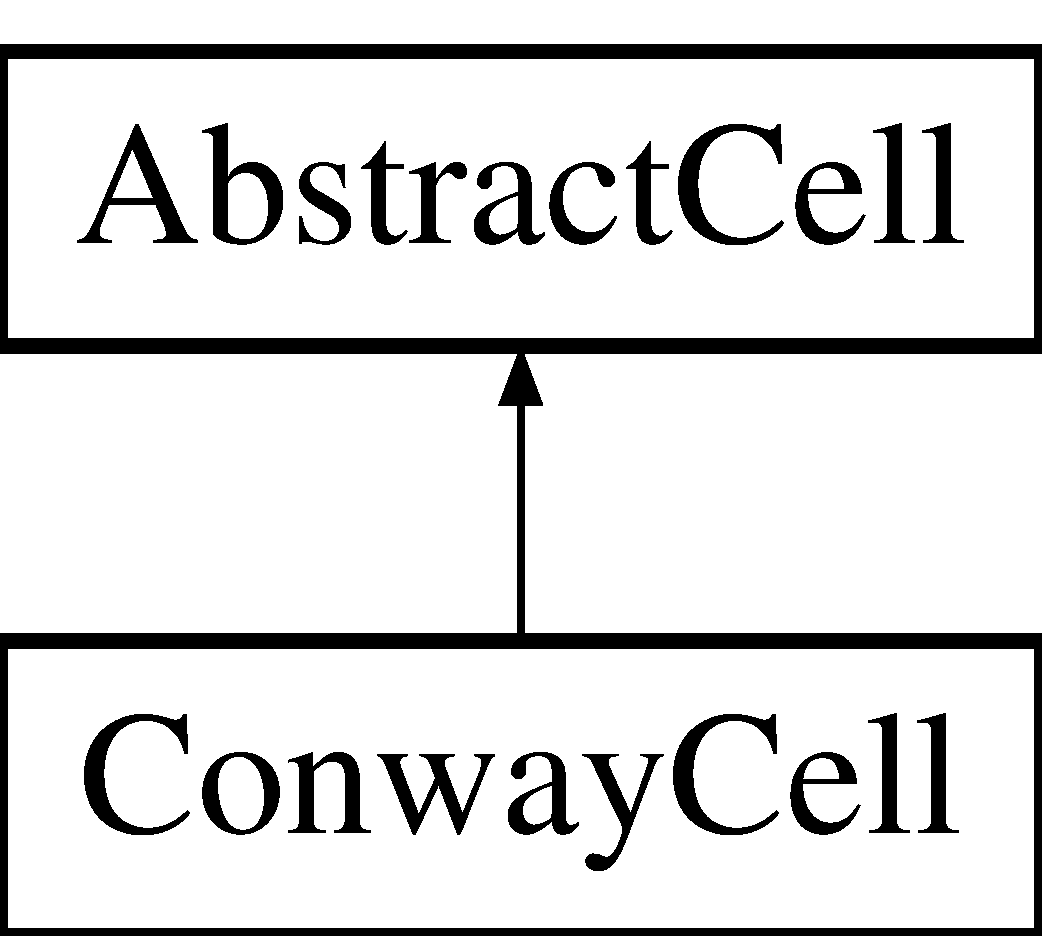
\includegraphics[height=2.000000cm]{classConwayCell}
\end{center}
\end{figure}
\subsection*{Public Member Functions}
\begin{DoxyCompactItemize}
\item 
void \hyperlink{classConwayCell_aec5f3637b37c4eef65cca5824bd0d6ce}{step} (int)
\item 
void \hyperlink{classConwayCell_a38780fdf3f4f4d5c5ed18fb732d428f7}{print} () const 
\item 
int \hyperlink{classConwayCell_ace1f4f79985ad1a375953f6da3fe0d6d}{get\-Cell\-Type} () const 
\item 
void \hyperlink{classConwayCell_aa1c5e99c5fbbc6d4fae3e70c03d412e2}{read} (char)
\item 
\hyperlink{classConwayCell}{Conway\-Cell} $\ast$ \hyperlink{classConwayCell_ab27dbaa286984ecbf77a35fbc742ea7f}{clone} ()
\end{DoxyCompactItemize}
\subsection*{Additional Inherited Members}


\subsection{Member Function Documentation}
\hypertarget{classConwayCell_ab27dbaa286984ecbf77a35fbc742ea7f}{\index{Conway\-Cell@{Conway\-Cell}!clone@{clone}}
\index{clone@{clone}!ConwayCell@{Conway\-Cell}}
\subsubsection[{clone}]{\setlength{\rightskip}{0pt plus 5cm}{\bf Conway\-Cell} $\ast$ Conway\-Cell\-::clone (
\begin{DoxyParamCaption}
{}
\end{DoxyParamCaption}
)\hspace{0.3cm}{\ttfamily [virtual]}}}\label{classConwayCell_ab27dbaa286984ecbf77a35fbc742ea7f}
Clones the cell 

Implements \hyperlink{classAbstractCell}{Abstract\-Cell}.

\hypertarget{classConwayCell_ace1f4f79985ad1a375953f6da3fe0d6d}{\index{Conway\-Cell@{Conway\-Cell}!get\-Cell\-Type@{get\-Cell\-Type}}
\index{get\-Cell\-Type@{get\-Cell\-Type}!ConwayCell@{Conway\-Cell}}
\subsubsection[{get\-Cell\-Type}]{\setlength{\rightskip}{0pt plus 5cm}int Conway\-Cell\-::get\-Cell\-Type (
\begin{DoxyParamCaption}
{}
\end{DoxyParamCaption}
) const\hspace{0.3cm}{\ttfamily [virtual]}}}\label{classConwayCell_ace1f4f79985ad1a375953f6da3fe0d6d}
Gets the cell type

\begin{DoxyReturn}{Returns}
-\/ \hyperlink{classCell}{Cell} type 
\end{DoxyReturn}


Implements \hyperlink{classAbstractCell}{Abstract\-Cell}.

\hypertarget{classConwayCell_a38780fdf3f4f4d5c5ed18fb732d428f7}{\index{Conway\-Cell@{Conway\-Cell}!print@{print}}
\index{print@{print}!ConwayCell@{Conway\-Cell}}
\subsubsection[{print}]{\setlength{\rightskip}{0pt plus 5cm}void Conway\-Cell\-::print (
\begin{DoxyParamCaption}
{}
\end{DoxyParamCaption}
) const\hspace{0.3cm}{\ttfamily [virtual]}}}\label{classConwayCell_a38780fdf3f4f4d5c5ed18fb732d428f7}
Prints the cell 

Implements \hyperlink{classAbstractCell}{Abstract\-Cell}.

\hypertarget{classConwayCell_aa1c5e99c5fbbc6d4fae3e70c03d412e2}{\index{Conway\-Cell@{Conway\-Cell}!read@{read}}
\index{read@{read}!ConwayCell@{Conway\-Cell}}
\subsubsection[{read}]{\setlength{\rightskip}{0pt plus 5cm}void Conway\-Cell\-::read (
\begin{DoxyParamCaption}
\item[{char}]{input}
\end{DoxyParamCaption}
)\hspace{0.3cm}{\ttfamily [virtual]}}}\label{classConwayCell_aa1c5e99c5fbbc6d4fae3e70c03d412e2}
Sets whether the cell is alive based on a char input 

Implements \hyperlink{classAbstractCell}{Abstract\-Cell}.

\hypertarget{classConwayCell_aec5f3637b37c4eef65cca5824bd0d6ce}{\index{Conway\-Cell@{Conway\-Cell}!step@{step}}
\index{step@{step}!ConwayCell@{Conway\-Cell}}
\subsubsection[{step}]{\setlength{\rightskip}{0pt plus 5cm}void Conway\-Cell\-::step (
\begin{DoxyParamCaption}
\item[{int}]{neighbor\-Count}
\end{DoxyParamCaption}
)\hspace{0.3cm}{\ttfamily [virtual]}}}\label{classConwayCell_aec5f3637b37c4eef65cca5824bd0d6ce}
Steps the cell forward one generation


\begin{DoxyParams}{Parameters}
{\em neighbor\-Count} & -\/ Number of neighbors the cell has \\
\hline
\end{DoxyParams}


Implements \hyperlink{classAbstractCell}{Abstract\-Cell}.



The documentation for this class was generated from the following files\-:\begin{DoxyCompactItemize}
\item 
Conway\-Cell.\-h\item 
Conway\-Cell.\-c++\end{DoxyCompactItemize}

\hypertarget{classFredkinCell}{\section{Fredkin\-Cell Class Reference}
\label{classFredkinCell}\index{Fredkin\-Cell@{Fredkin\-Cell}}
}
Inheritance diagram for Fredkin\-Cell\-:\begin{figure}[H]
\begin{center}
\leavevmode
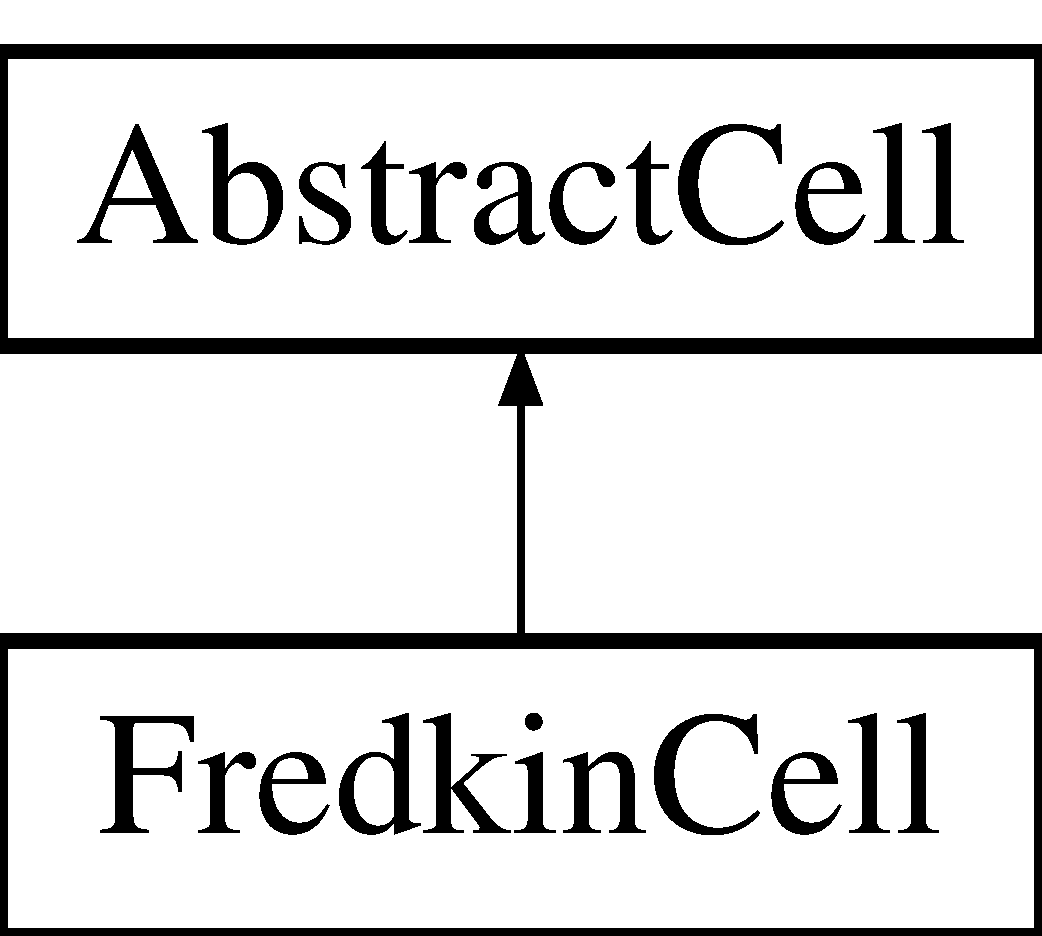
\includegraphics[height=2.000000cm]{classFredkinCell}
\end{center}
\end{figure}
\subsection*{Public Member Functions}
\begin{DoxyCompactItemize}
\item 
\hypertarget{classFredkinCell_a5ae41bba71089226e67e3d49ee5533d9}{bool {\bfseries needs\-Transform} ()}\label{classFredkinCell_a5ae41bba71089226e67e3d49ee5533d9}

\item 
\hypertarget{classFredkinCell_ae75fa4394227223f96d643d850ac2027}{void {\bfseries step} (int)}\label{classFredkinCell_ae75fa4394227223f96d643d850ac2027}

\item 
\hypertarget{classFredkinCell_a344bdea2238bb65b7d5013cf9359b3f5}{void {\bfseries print} () const }\label{classFredkinCell_a344bdea2238bb65b7d5013cf9359b3f5}

\item 
\hypertarget{classFredkinCell_ab550b7553cb649799f7c286369732527}{int {\bfseries get\-Cell\-Type} () const }\label{classFredkinCell_ab550b7553cb649799f7c286369732527}

\item 
void \hyperlink{classFredkinCell_a0a849ac1b7b8620429b2f5c139043e87}{flip} ()
\item 
\hypertarget{classFredkinCell_a92300644207f5fc72f9e44584acf7a18}{void {\bfseries read} (char)}\label{classFredkinCell_a92300644207f5fc72f9e44584acf7a18}

\item 
\hypertarget{classFredkinCell_a26ab307f5839cb7a7cf8d97ea27162f7}{\hyperlink{classFredkinCell}{Fredkin\-Cell} $\ast$ {\bfseries clone} ()}\label{classFredkinCell_a26ab307f5839cb7a7cf8d97ea27162f7}

\end{DoxyCompactItemize}
\subsection*{Additional Inherited Members}


\subsection{Member Function Documentation}
\hypertarget{classFredkinCell_a0a849ac1b7b8620429b2f5c139043e87}{\index{Fredkin\-Cell@{Fredkin\-Cell}!flip@{flip}}
\index{flip@{flip}!FredkinCell@{Fredkin\-Cell}}
\subsubsection[{flip}]{\setlength{\rightskip}{0pt plus 5cm}void Fredkin\-Cell\-::flip (
\begin{DoxyParamCaption}
{}
\end{DoxyParamCaption}
)\hspace{0.3cm}{\ttfamily [virtual]}}}\label{classFredkinCell_a0a849ac1b7b8620429b2f5c139043e87}
Flips the alive flag of the cell 

Reimplemented from \hyperlink{classAbstractCell_a2adb986c55c4ed6613549ff011fb8d25}{Abstract\-Cell}.



The documentation for this class was generated from the following files\-:\begin{DoxyCompactItemize}
\item 
Fredkin\-Cell.\-h\item 
Fredkin\-Cell.\-c++\end{DoxyCompactItemize}

\hypertarget{classLife}{\section{Life$<$ T $>$ Class Template Reference}
\label{classLife}\index{Life$<$ T $>$@{Life$<$ T $>$}}
}
\subsection*{Public Member Functions}
\begin{DoxyCompactItemize}
\item 
\hypertarget{classLife_aa481017182766d2228023c08eeb2ccca}{{\bfseries Life} (int width, int height)}\label{classLife_aa481017182766d2228023c08eeb2ccca}

\item 
\hypertarget{classLife_ad096847c1b28d71138a2b689621cb50d}{void {\bfseries step} ()}\label{classLife_ad096847c1b28d71138a2b689621cb50d}

\item 
\hypertarget{classLife_ab7ab112da0a3584ee96f6746bc59ea6b}{void {\bfseries read\-Input} (char in, int position)}\label{classLife_ab7ab112da0a3584ee96f6746bc59ea6b}

\item 
\hypertarget{classLife_a229482838bcef44942bcc64264210613}{void {\bfseries print} ()}\label{classLife_a229482838bcef44942bcc64264210613}

\item 
\hypertarget{classLife_a3cf66fe8e6e614c4a17874cc4744921f}{int {\bfseries get\-Population} () const }\label{classLife_a3cf66fe8e6e614c4a17874cc4744921f}

\item 
\hypertarget{classLife_af3a454b69c71826cfd971e2cafa1ee97}{int {\bfseries get\-Neighbor\-Count} (int position) const }\label{classLife_af3a454b69c71826cfd971e2cafa1ee97}

\item 
\hypertarget{classLife_a971c586958f37ef55b2d21793b3de430}{T $\ast$ {\bfseries at} (int index)}\label{classLife_a971c586958f37ef55b2d21793b3de430}

\item 
\hypertarget{classLife_a00e3429d347f06866100ad3c53922324}{T $\ast$ {\bfseries at} (int index) const }\label{classLife_a00e3429d347f06866100ad3c53922324}

\item 
\hypertarget{classLife_a7d9aadc616c6577e10f6bc7849dd9432}{T $\ast$$\ast$ {\bfseries begin} ()}\label{classLife_a7d9aadc616c6577e10f6bc7849dd9432}

\item 
\hypertarget{classLife_aed86fa5bbb55e45bf7723aad63949efc}{T $\ast$$\ast$ {\bfseries begin} () const }\label{classLife_aed86fa5bbb55e45bf7723aad63949efc}

\item 
\hypertarget{classLife_ae597f61db6246f7e1e04a1f51a0c39fe}{T $\ast$$\ast$ {\bfseries end} ()}\label{classLife_ae597f61db6246f7e1e04a1f51a0c39fe}

\item 
\hypertarget{classLife_a6abb69bbd7bbc24f7ea4e1f2a8d7f008}{T $\ast$$\ast$ {\bfseries end} () const }\label{classLife_a6abb69bbd7bbc24f7ea4e1f2a8d7f008}

\end{DoxyCompactItemize}


The documentation for this class was generated from the following file\-:\begin{DoxyCompactItemize}
\item 
Life.\-h\end{DoxyCompactItemize}

%--- End generated contents ---

% Index
\newpage
\phantomsection
\addcontentsline{toc}{chapter}{Index}
\printindex

\end{document}
